\chapter{Implementation}
\label{chap:imp}
\lhead{\emph{Project Implementation}}
This chapter should comprise 15 pages and enumerate your experience when doing what you wanted to do the way you wanted to do it. 

\section{Difficulties Encountered}


 \item \textbf{Easy}
 \item \subsection{ \textbf{Camera not working } }

\item Technical difficulties where encountered throughout the implementation phase when trying to use my laptops camera in order to capture my face, this issue only occurred during the beginning of the my implementations and was easily fixed with a little troubleshooting, this issue could have been a highly fatal to the completion of my drowsiness detection system as this system is solely dependent on a working camera to capture and monitor facial features and cues from individuals exhibiting drowsiness.
  \begin{enumerate}
  \item This issue didn't have any effect on the architecture of my solution due to this being an external issue with the windows operating system.The camera wasn't updated to the latest version and was most likely clashing with the most up to date version of windows 10.
 \item This issue had a very high risk of disrupting the completion of my project as my project is very dependent on using a working camera in order to be able to perform successful facial behavioural capturing, to detect eye closure being exhibited by the individual.                                     		\item The methodology being used wasn't effected as this problem wasn't significant enough to cause any drastic methodology changes with the development of the system going forward, the only manner in which this issue may have caused an effect on the methodology that I was if this issue was in any way fatal as a complete new alternative would have to be deduced in order to progress with the drowsiness detection system. 		\item The implementation schedule was halted for a short period in order to get the camera working again, this period was significant and was majorly temporary, the implementation schedule was only halted for a week in order for me to search for a solution.                                                      
 \item The evaluation plan wasn't effected because this issue fit within the means of my project evaluation that was outlined in chapter 4, by knowing that if this issue persisted then my evaluation of a successful project would have been effected severely.															 
 \item  The first step I took when I faced this problem was to initially check if I gave pycharm permission to access my camera, when I went about ensuring if it was and then realising this wasn't the reason for the issue I then went ahead and looked at opencv forums searching for problems that other individual had that where similar to my own camera problem. I ran through these issues and they where majority coding errors, looking through these coding solutions to the the coding errors that others have experienced I copied and pasted some solutions just to check if I may have have been incorrect in my coding structure I opened a separate script to check still without any success, so from that I had deduced that is may either be a hardware issue or an issue to do with the operating system, In order to resolve this issue I found myself accessing the device manager within my computer and uninstalling and reinstalling the camera software onto my computer, then followed by a quick update, this didn't resolve my issue and I in turn found the solution by looking up the computer model and downloading the and installing the latest driver for my my camera online through google which then resolved my issue 																										
 \end{enumerate}

\item \subsection{ \textbf{Pycharm facial detection technology } }
\begin{enumerate}																																																								\item initially PyGaze was a technology that I attempted to use to capture and recognise facial cues  and behaviours, but difficulties where had trying to translate the information captured by the open source technology into information that could be understood by the python script, I then in turn switched to an open source XML import that would do the facial detection for me and could be easily understood and manipulated using python code.
\item This issue effected the design of the system slightly as I switched from open source technology to an an open source XML script.
\item The architecture was changed slightly as the open source eye tracking technology was discontinued and open source XML  was introduced which carried out all the facial, eye and mouth detection requirement
 \item It could have represented a major risk to my project if I wasn't able to find an alternative approach to the then there could have been a serious risk in the detection aspect of the system and could have resulted in a failed system.
        \item This didn't effect the methodology as I approached this problem exactly as the methodology outlined I should, by revising the my approach and taking notes of any problems and solutions to those problems 
        \item It changed the implementation schedule slightly but I remained on track as this problems solution was found and used resolve the problem very quickly.
        \item This didn't change the evaluation plan that I was using to determine successful and unsuccessful progress to the goals that I had outlined to complete.
    \item I looked open source opencv facial detection technology and quickly found a very common method that was used for facial detection systems.
    \end{enumerate}

\item \textbf{Medium}
\item \subsection{ \textbf{ Wi-Fi connection problems } }																																									\item Once my working environment was forcefully changed due to the Coronavirus all work that being done on the drowsiness detection system had to be done from home on an unreliable Wi-Fi connection, random connection losses would randomly persist and could halt any progress being carried out trying to troubleshoot errors in my code structure and logic, when good progress was being made an abrupt connectivity would interrupt that progress, connectivity loss could last up for a couple of hours and  could sometimes result in the loss of a full days work and progress.	                                                            																																                                              \item This issue was persistent and as it was evident more towards the end of the semester causing alot of the design to be implemented in a short space of time.												
\begin{enumerate}
 \begin{enumerate}
        \item The blackboard design pattern wasn't used due this issue solely as there was too many errors being displayed with its                implementation with the original solutions that I had developed initially, as well as a highly complicated structure that takes long periods of time to fully inter grate alongside my solutions for my drowsiness detection system
        \item It did possess somewhat of risk to the completion of my drowsiness detection system as there was a chance that not enough work could  have been completed before the very final deadline.
\itemThe methodologies that where outlined in chapter 4 wouldn't need to be changed due to this, the approach going forward was the same as I was using a scrum approach there wasn't any necessary need to change the methodology only to evaluate the situation and then to modify my approach implementation approach for it.  
 \item It slowed down my implementation schedule, which in turn forced me into spending less time developing the system itself this was because the window in which I could work on the system was random, although this issue happened it wasn't very frequent making it impossible to work on the system.																																														\item The evaluation plan wasn't effected because this issue fit within the means of my project evaluation that was outlined in chapter 4, if this issue persisted to the point where there was no way to to work on the system it may have effected my decision making in the evaluation of my developing the goals at the time and the final goals of the system itself
 \item In order to overcome the difficulties of this I made sure to download videos off of YouTube in case i needed to reference opencv tutorial to help achieving certain tasks that would have been required to full fill objectives and my weekly tasks, as well as taking screenshot of the OpenCV documentation using word .
   \end{enumerate}

\item \textbf{Hard}
\item \subsection{ \textbf{Caronavirus Pandemic} }																																										\item The Covid-19 pandemic was a difficulty that was encountered mid way through my project implementation, not only has this effected me but the people that I cared about around me which in turn resulted in unnecessary stress and a period of adaption. The pandemic also affected my work environment and schedule, when I had access to collage facilities the rate in which I was able to finish my drowsiness detection system was moving ahead smoothly as I had access to the collage library which had computers with a reliable internet connection, I also had access to a quite area where I could spend time performing tasks that I had planned for the week to do on my drowsiness detection system.due to the carnivorous pandemic sweeping over the world and the nation so abruptly. cases where rapidly increasing it has brought alot of uncertainty to collage progression, self isolation and environmental restriction brought into effect by the government caused for an experience that was surreal which caused panic   																																																										\item It effected the original design of the project immensely,being forced to work from home with horrible internet connections and unnecessary distractions this limited the final database functionality severely. 																																				\item It did have the biggest risk to the completion of the project because there was a high chance that I could have contracted the virus if that ever possibly happened then it could have prevented me from 	completing the system before the deadline the virus out of control and wasn't full contained by the government, although contact tracing and other procedures where carried out this wasn't enough to stop the spread.						\item It affected my weekly reviews of my progress initially until I was able to get back on track with my own weekly personal weekly reviews and overviews of the work done up the point.																																													\item It had a major effect on the implementation scheduler that I was following up until the Closure of the collages for the remained of the semester which brought on horrible connectivity issues, and an unsuitable environment to complete tasks, this took quick self adaption to get back on schedule																																																										\item The evaluation plan was slightly altered as the final system that was originally planned wouldn't be completed and I had to make do with lesser overall database functionality.																																															\item Managing the difficulty that had arisen was very difficulty to do as the Caronaviruse still  Continuous persists in Ireland and globally showing no signs of letting up, but managing other factors that where related to it such as bad Wi-Fi and bad work environment can be overcome as it is far easier to research ways to improve your work environment or to call the internet service provider in order to fix issues with the connection by bringing it to there attention.
\end{enumerate}
	


\section{Actual Solution Approach}
In December of last year, when writing the first version of the report, in Chapter 4 you came up with your original solution approach. On it, you presented (i) the architecture of your solution, (ii) your list of use cases, (iii) a risk assessment, (iv) a methodology to develop your solution approach, (v) your implementation schedule, (vi) your evaluation plan and (vii) some prototype of the resulting product. From January to April you have been developing your solution approach. Along the way you have encountered difficulties (the ones listed in Section 5.1) which might have modified your original plan so that you can come up with an actual developed project.

This section is effectively the production of "as built" specification where you compare your original design to the final finished project. Please go section by section (the ones listed from (i) to (vii) in the last paragraph. For each section, enumerate any difference between the original design and the final project, and justify the difficulty forcing you to make such this change. Do not fret if some of these changes are radical, what is important here is that there is a clear rationale for changes made.
[By the end of December of last year I had an initial understanding of the opencv library and a basic understanding and design of the architecture that  I thought was enough to successfully to build the drowsiness detection system, some design outcomes in the research phase have been used in the implementation phase which is a sign of good research carried out previously and some outcomes that where researched and found to be of no use within the final implementation build, overall I will be detailing my progress through the implementation phase and comparing the final solution to the research phases architecture and final conclusions, both overall outcomes will be compared under a number of factors, like architecture ,use case , methodology , implementation schedule, evaluation plan and prototype,  all these will be the premise from which I will be detailing my solution approach

\subsection{Solution Architecture}
\subsection{Design Model}
During the research phases I specified my architectural specification of the drowsiness detection system I said I would be modelling the system using a blackboard design pattern, however when developing my system I had issues  implementing this design pattern as it was too complex for the time required, choosing this design model  at the time suited the type of system that I was designing  as it suited the needs of the system as it was heavily recognition focused. The blackboard design pattern would typical be used solely for speech recognition but when it came to developing my drowsiness detection system I intended to use it for the for the user identification aspect of the system.  When designing the solution I initially attempted to fit the  blackboard skeleton into my code but encountered issues when it came to capturing a new frame and storing it as an image in a directory in order for the system recognise the individual from the image. 

\subsection{Technologies}
When I first did my research on the  technologies that I would have been using in the the development phase my research was very accurate as almost all the technologies where used.When i was developing the system I had to use other technologies within the project itself to successfully achieve the goals and ambition that I had going forward. The main library that was used in the solution approach was the OpenCV and this library was essential in carrying out facial detection, video capturing and facial recognition in the project. The interface that the OpenCV was used with was the the python language this was specified in chapter 4, methods that where specified in where used to do exactly as was specified within the research phase, methods like the VideoCapture and read() where both utilized thorough out the development of the drowsiness detection system .
 Haar cascade classifiers where used to detect the face and eyes of the individual, there where multiple unique types of harrcascade scripts that performed different types of detection these scripts where used simultaneous, parallel to each other in order to perform eye detection face detection and detection when glasses where on the individual, during the implementation i used methods dedicated to reading Haar cascade files OpenCV had a built in algorithm called CascadeClassifier that would access the cascade file using CascadeClassifier(‘ path to our Haar cascade XML file’)  this process within the system was always accompanied by a detectMultiScale(gray) this was used to perform grey scale capture as the computer processor can only differentiate  shades of darkness, the detectMultiScale(gray) method is in place so that it can return an array of detection which consist of numerical values that are plotted on an x and y axis without the capture being converted to grey scale the computers processor wouldn't be able to detect differences in in each frame this is all done so that the system create a region of interest.
 

\subsection{Database}
A back end database was one of the intended functionality requirements to be in place when the research concluded in December, Firebase  was the database that was decided upon to add backend administrative functionality to the system the idea was to have an administrator monitor over the drivers and to detect if the driver was sleepy and showed signs of drowsiness, assess the state in which the drivers was performing on the road.  The purpose of the database was to save the state of the driver in order for it to be referenced by the Drowsiness detection system so as to keep track of which current drivers are feeling drowsy and to send an alert to the driver to inform the driver that he is exhibiting too many instances of drowsiness and that he must take a break or, goal of the database was to have all the details that where unique to the driver  such as first and last name accompanied by his driver id number. In the final system i was only able to capture the number of times a driver was feeling drowsy and to upload it to the database, this is far from the database functionality that was envision in December this lack of database functionality was mostly due to the covid-19 pandemic that altered and slowed down the development schedule.

\subsection{Framework}
In December I decided upon Python as the language that will be used as it was commonly know as a general purpose language and was accompanied by many libraries and tools that are designed for a wide range of unique projects. The usefulness of Python was evident as an excellent language and was the perfect choice for implementing  architecture of this system. Python is well know for its  backend web development its artificial intelligence and the scientific computing frameworks is possesses, as I designing this system their was huge emphasis on artificial intelligence the haar cascade classifiers scripts that where used to detect a face being displayed in the webcam,  implementing  these scripts where easy, opencv has methods which support external cascade XML imports.  The final design consists of  a single python scripts that will communicate  with multiple haar cascade XML imports which each other, their is  multiple methods Dedicated to reading the input from the camera and converting each frame to a grey scale copy which is then be accompanied by a script that reads and implement Haar Cascade classifiers algorithm on the frames received of the face and the eyes, their is a method that implements a cascade file which detects a if individuals has blinked which is then proceeded with an alarm. 

\subsection{Hardware failure 1.1}
A risk that did occur in this project was an initial hardware failure that was the camera not working initially preventing   halting initial work  trying to develop my project  if this issue persisted during my implementation phase of this system, it presented a risk that would stop my project from being fulfilling  the  core functionality requirements of the system thankfully this issue was resolved and i was able to progress with developing my system. This was an  issue touched upon in the research phase as I said if this occurred in relation to  their being a hardware failure their could be a high possibility of a  complete system failure occurring, loss of  implementation's progress was also stressed and depending on which Stage i was at I  could have lost all my progress. This wasn't a  common risk but a very reasonable on and this predictive thinking helped  insure a  there wasn't a complete system failure during the collage semester and through out the implementation. This type of risk was easily avoided by the use of  GitHub allowing me to commit each work cycle  in the event of a system failure any as if this happened i could access me work  using any other computer to access my my repository and work can be continued on the system where I have left it before the system hardware failure.

\subsection{Software failure 2.1}
Another risk that did occur during the development was a software failure which required a change in design from a eye tracking open source software to a XML import file to continue  my progress to developing the system, if I perhaps couldn't find an alternative then developing this system would have failed, in December i predicted that certain libraries I planned on using for this project may not have been compatible with the hardware of my computer but in actuality it was the open source eye tracking technology that caused the issue and if this issue persisted then a major risk in the implementation phase of the system was evident, ""\textbf{This can be a major issue if I encounter this during development as I could have to re-decide how I will re-implement my project and can hinder progress cutting time off of the remaining time that I have left when I have to fully develop my project}"" these are the exact words that I used in  the case this happened through the implementation phase . Luckily when doing my research i had found multiple directions I could have taken to fully complete the this assessment and when my initial direction didn't work I changed to an alternative method which took a little longer to grasp and implement . 
\subsection{Requirements 4.5}
As the development of this system was self managed by myself there was risk of the requirements being in-adequately defined and undertaken by myself during the implementation phase of my project. During the implementation phase I discovered a requirement changes and functionality additions such facial recognition using in built facial trainer and instances where tasks became unnecessary due to time constraints such as a backend database during implementation when this happened work around where though of and implemented such as to equal the weight of functionality lost for the removal of a database, facial recognition was added as a counter balance because this core  requirement  change in this system produced  difficulty. Requirement change wasn't expected to show up in December, my expectation of this was very rare at the time but this is now not the case .Their was decisions made on my end to change functionality of the system, and this came down to lack of time forcing drastic changes which has had a big impact on the  the system. 
\section{Methodology}
The waterfall model was used as It was the most popular development methodology when researched upon and used in large parts of the industries,  it is used in parallel using an agile technique.  The model allowed for far easier testing  and analysis through out the development of my system. The Agile development methodology used to continually allocate my work into a cycle and to continuously evaluate successful sprints at the end of each cycle, i allocated myself mostly a week to perform each task that i had in my schedule and in the case it took longer at the evaluation phase i would then proceed allocate more time in the next sprint to accomplish the previous task and the following task.   It was an approach that I found  suitable  for adaptation through out development of the system. The implementation of this methodology allowed  for adaption in the later stages of developments change deviation at these stages can be damaging  that can occur and but the time heavy cycles can create opportunity to implement other functionality this caused the  outcomes not to be clear. The scrum programming  methodology is the methodology that I used to implement functionality, each iteration is a cycle of one week self management and organisation is needed and this made the scrum suitable through out the development system
  

\subsection{Implementation Schedule}
This was the schedule I  planned  and followed during the implementation phase within the research phase,  is to use the  duration  of  the second semester, and the time allowed to me wisely. The approach taken to make sure this project is completed is an iterative and incremental this has already been dictated by the methodologies section where I have discussed this earlier. Each of my increments we done  in equal time duration from each other.  Below I have listed all the tasks that I plan to do from the beginning to the end this should Provide the right type idea how my project implementation will be progressed from the beginning cycle until the end

\begin{itemize}
\item Task 1 - Install all the required software and technologies that my system will require for example PyCharm, PyGaze, OpenCV and install Firebase into working environment.
\item Task 2 - Configure all the technologies so that my working environment has all the technologies present and running the correct version. 
\item Task 3 - Download the blackboard design model script and Begin implementing OpenCV Methods and class can work start making use of the camera components on my computer. 
\item Task 4 - Perform frame capturing functionality so to convert these frames into grey scale so that the Haar cascade classifier algorithm can start to do facial recognition 
\item Task 5 -Begin developing Haar cascade classifiers algorithm in order to use the algorithm to identify I users face.
\item Task 6 - Once developed train the algorithm start identifying a users face in each frame that is captured. 
\item Task 7 - Once the Haar cascade classifier has been trained to detect faces from each frame that is extracted of the users face then begin to train the Haar cascade classifier algorithm to detect the users eyes.  
\item Task 8 - Finally by using the Perclos algorithm to calculate the eye open to eye close ratio an score can be retrieved so that an threshold can be configured in order to detect if a user is feeling sleepy. 
\item Task 9 - Configure Alarm functionality with the speaker components on the on the computer so that when the threshold has been exhibited by the driver then the alarm will be sounded.
\item Task 10 - Begin database implementation to the system and this will be one of the final tasks to be done.
\item Task 11 -Set up JSON script inside the FIREBASE database with parameter consisting of the users details and drowsiness ratio 
\item Task 12 - Configure the serialization of data from the system to the backend database 
\item Task 13 - When drowsiness occurs with the driver then the admin monitoring the Database will be informed
\item Task 14 - Final test of the the system will be done to ensure the requirements have been met.
\item Task 15 - Provide comments and explanations of what the code does, tidy up the code in area need tidying up. 
\end{itemize}

\section{Evaluation }
 At the end of my development my evaluation had changed as  some of the goals that i had and objectives where changed, what was achieved  quickly was evaluated and noted by the successful output of the system, while others objectives need  some considerable  planning to develop work around that where considered sufficient  evaluated outcomes .  When  i performed my planning  for these tasks to be developed evaluation conditions had to be implemented along with them to have efficient outcomes. These goals where maintained by a time bracket as was specified  by the scrum the time bracket allowed me to measure the progress of each goal, simplification of the task ensured that it provided easily understood value. My final evaluation can be seen as a success as the main core functions have been achieved the evidence is the alarm being triggered when my eyes are closed and what was  not  a success within this project such as  the database  is evident because database functionality is missing .By understanding this i understood what i wanted to  achieve, this understanding was the core  evaluation factor i needed to perform my evaluative measure to having a successful outcomes at the end of my development. Other evaluation techniques where used to determine if the system was doing tasks correctly such as threshold the detection  parameters to suit the needs of the the system efficiently.


\section{Prototype}
Although no implementation has been done yet I carried out a few test with some of the libraries using OpenCV.

The first Test I carried out was a simple library test to see if OpenCV worked. I wrote a small script.

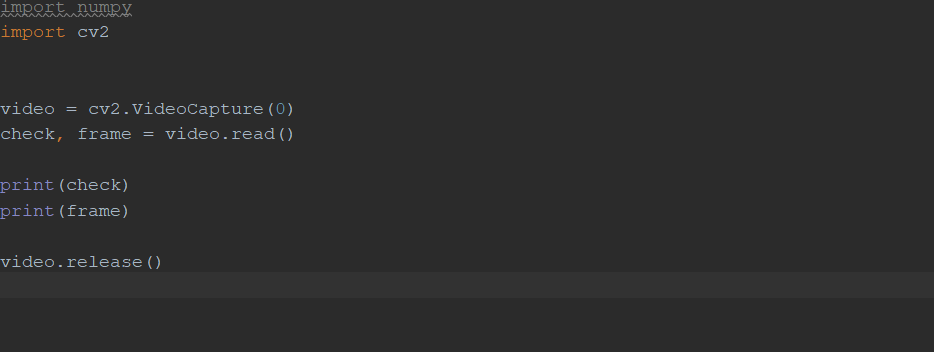
\includegraphics[width=0.8\textwidth]{Figures/Pythonscript.png}

This was the first Python script that I ran.  I ran this script so that I can observe what the terminal would output and a received what I expected from the terminal, which was matrices with zeros residing inside them. The reason They are displaying zero is because  the camera isn't active and isn't picking up any frames.

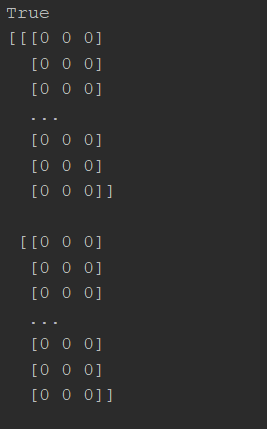
\includegraphics[width=0.8\textwidth]{Figures/terminalPythonScript.png}

This above image will show you what I the output received when I ran the script, you will see multiple matrices with zeros residing within them as i outlined before. 

I then updated my script so that I can have the camera show up on my screen although the camera is turned off by default in my setting this script shows that the OpenCV library methods are communicating with with my computer and very efficiently also.

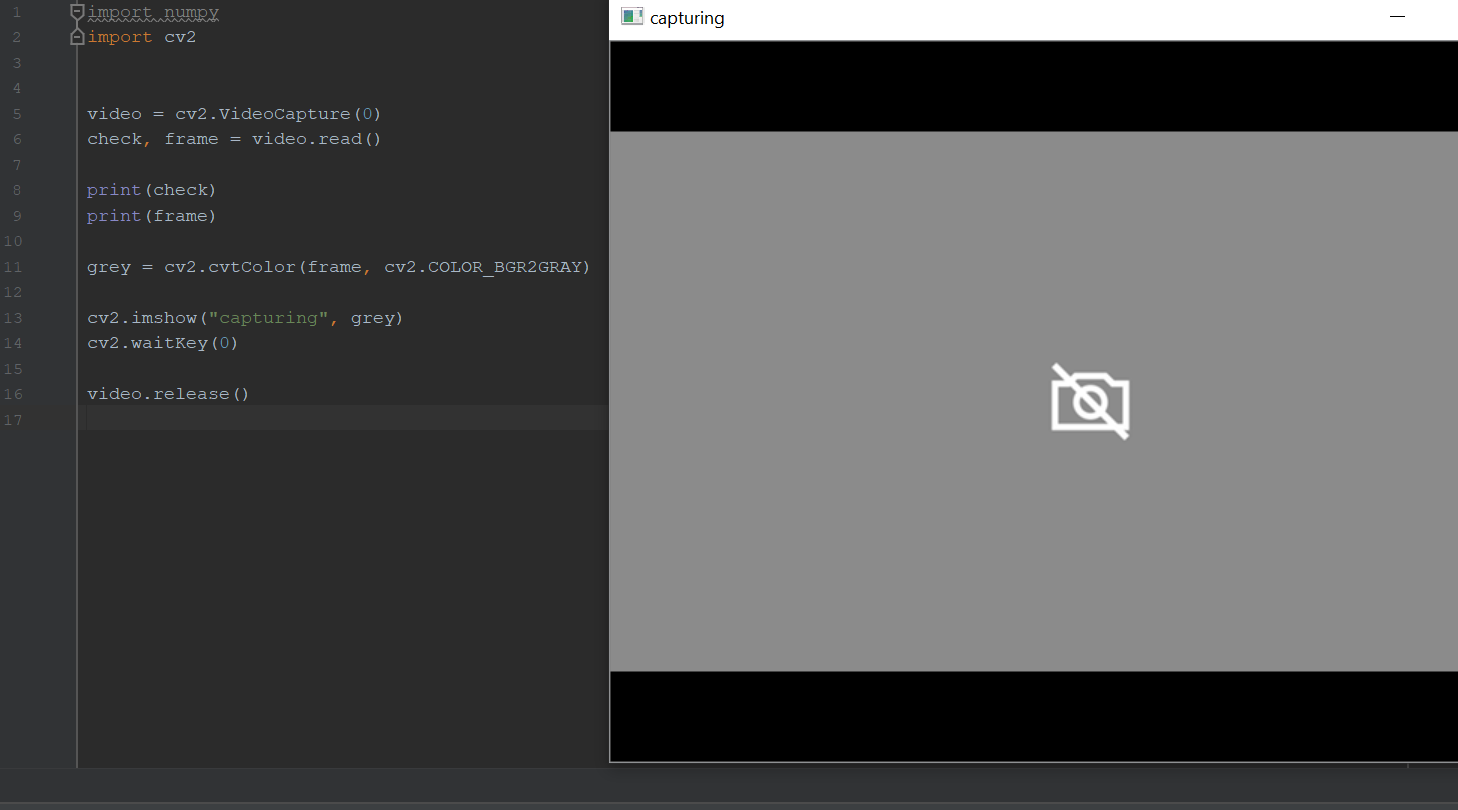
\includegraphics[width=0.8\textwidth]{Figures/Pythonscriptwithcamera.png}

AS you can see I have added a few more methods and have used a method to convert each new frame to grey scale this cant be seen as their is new picture but the functionality is within the code.

]
















